\section{Results}


\subsection{Effective multiplication factor}
Figures~\ref{fig:keff}, \ref{fig:keff_zoomed} show the effective multiplication factors. 

\begin{figure}[ht!] 
  \centering
  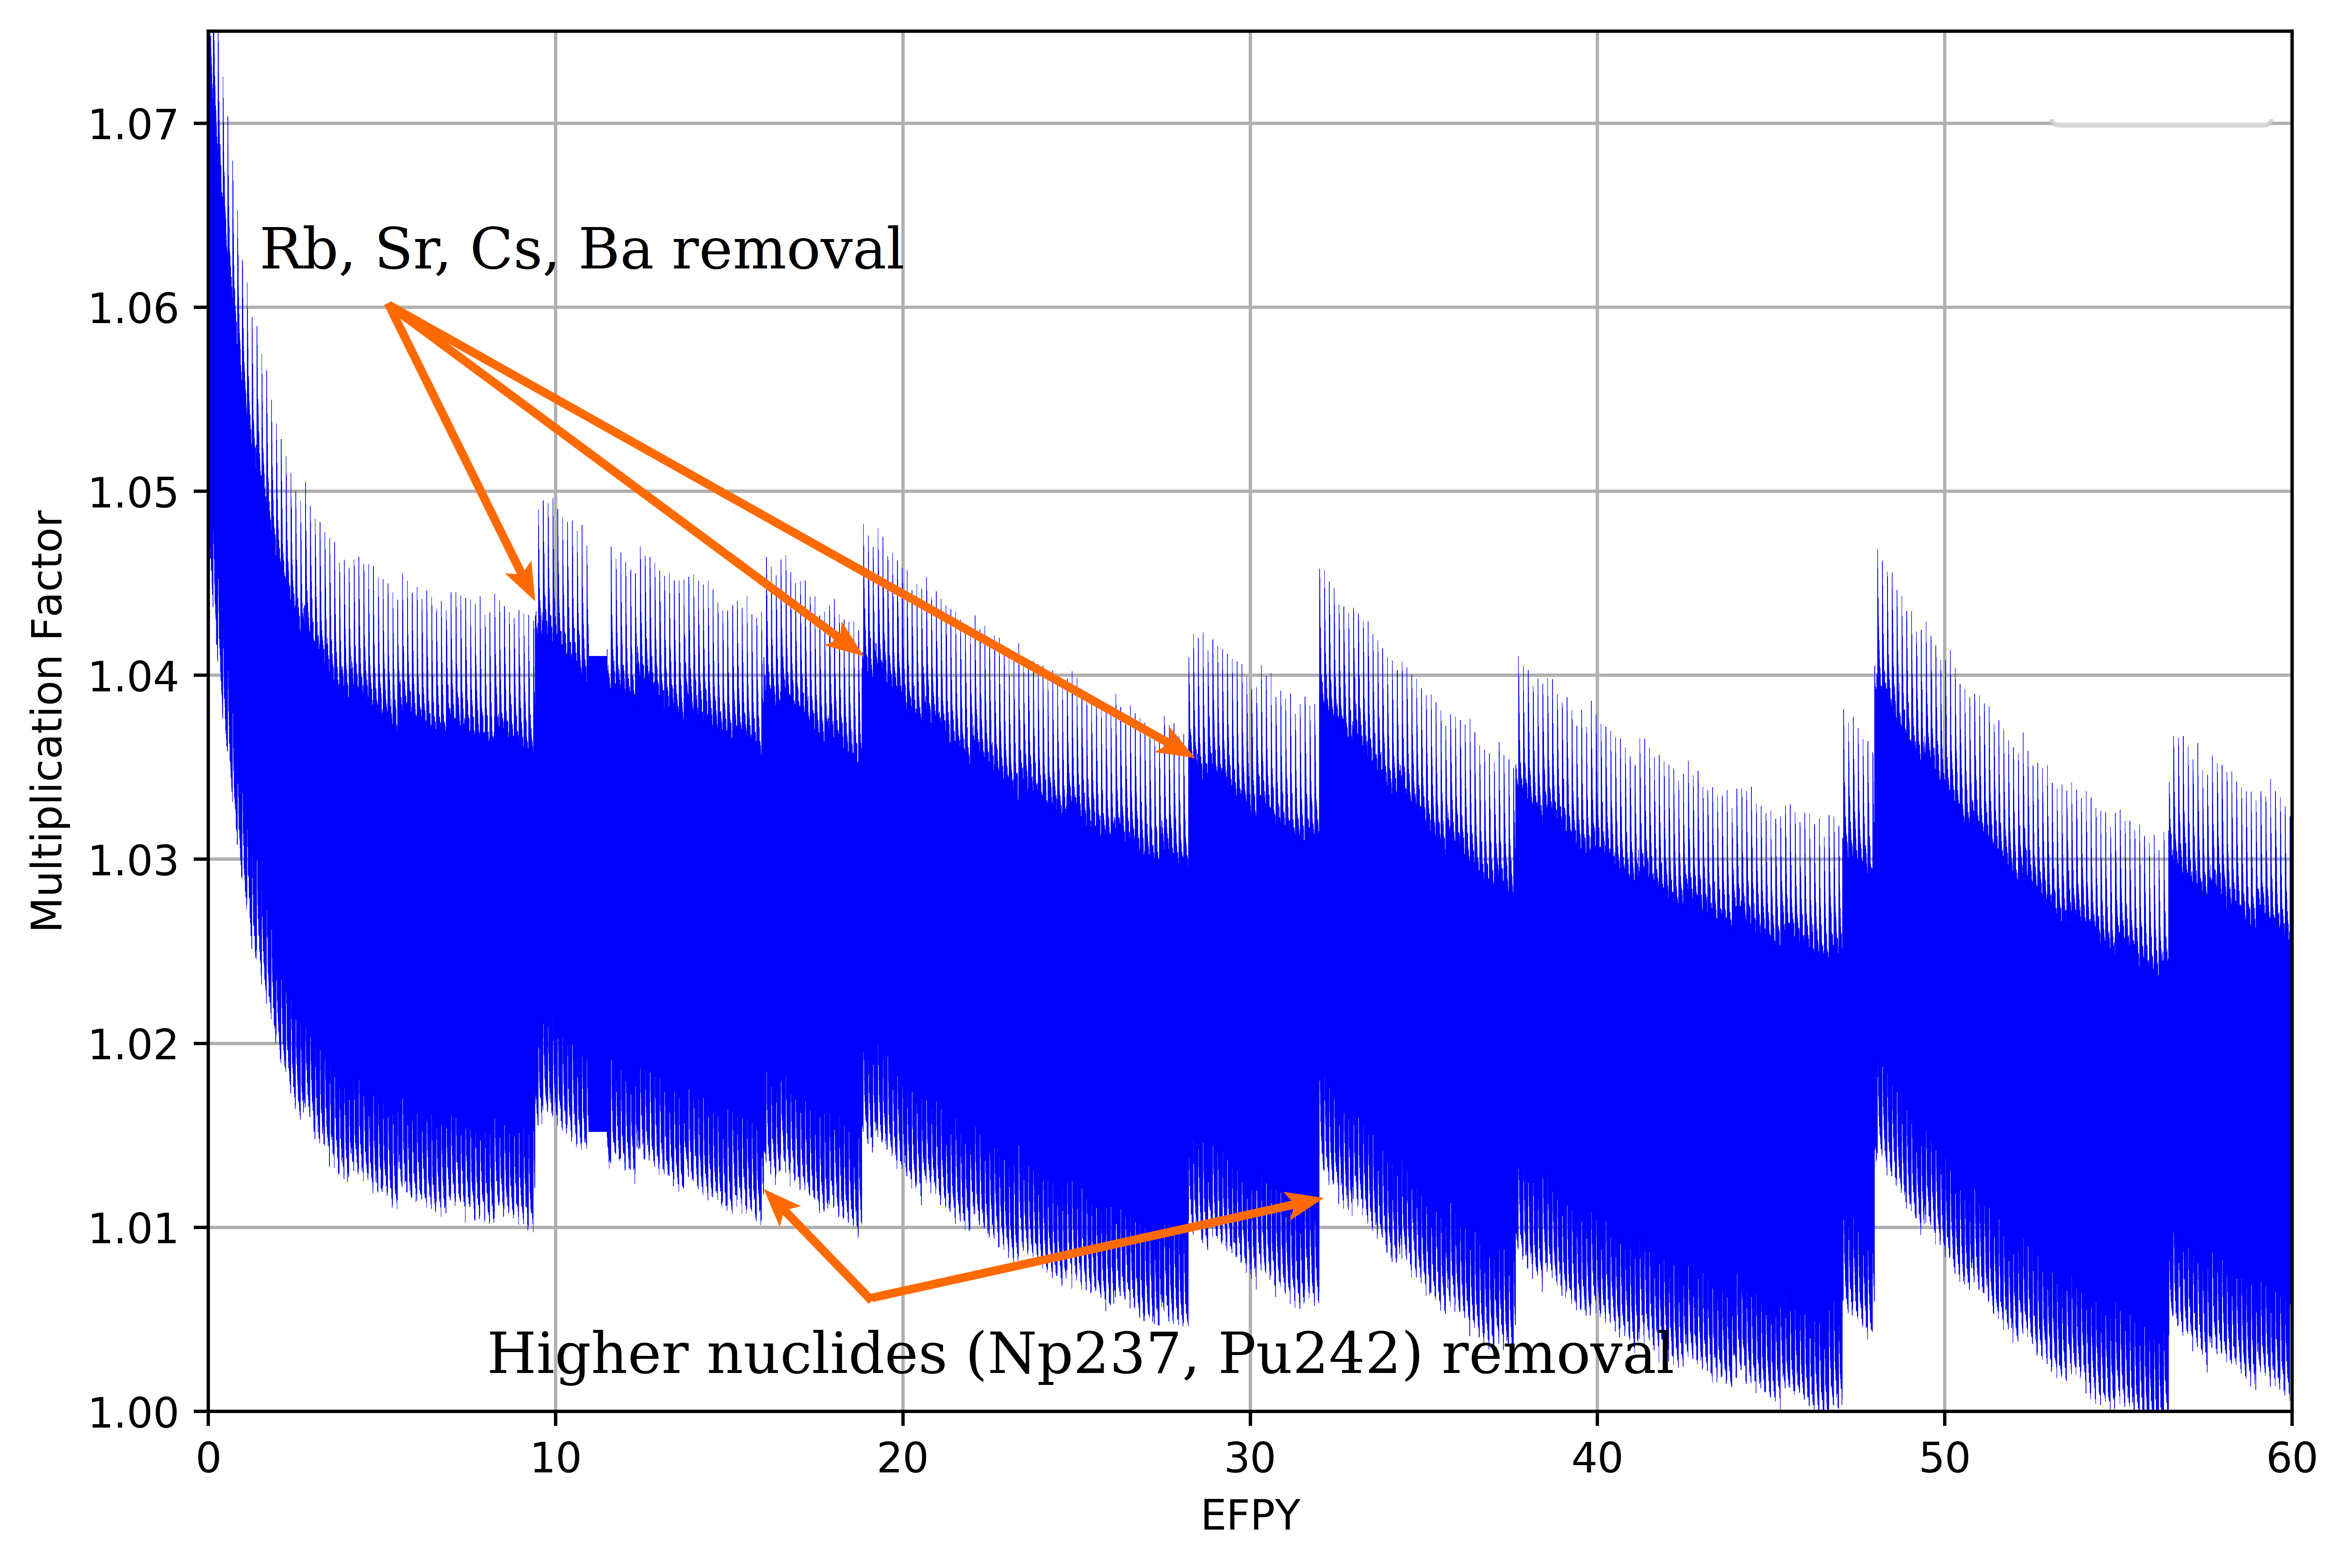
\includegraphics[width=\textwidth]{keff.png}
  \caption{Effective multiplication factor dynamics for full-core \gls{MSBR} 
  model over a 60-year reactor operation lifetime.}
  \label{fig:keff}
\end{figure}
\begin{figure}[ht!] 
  \centering
  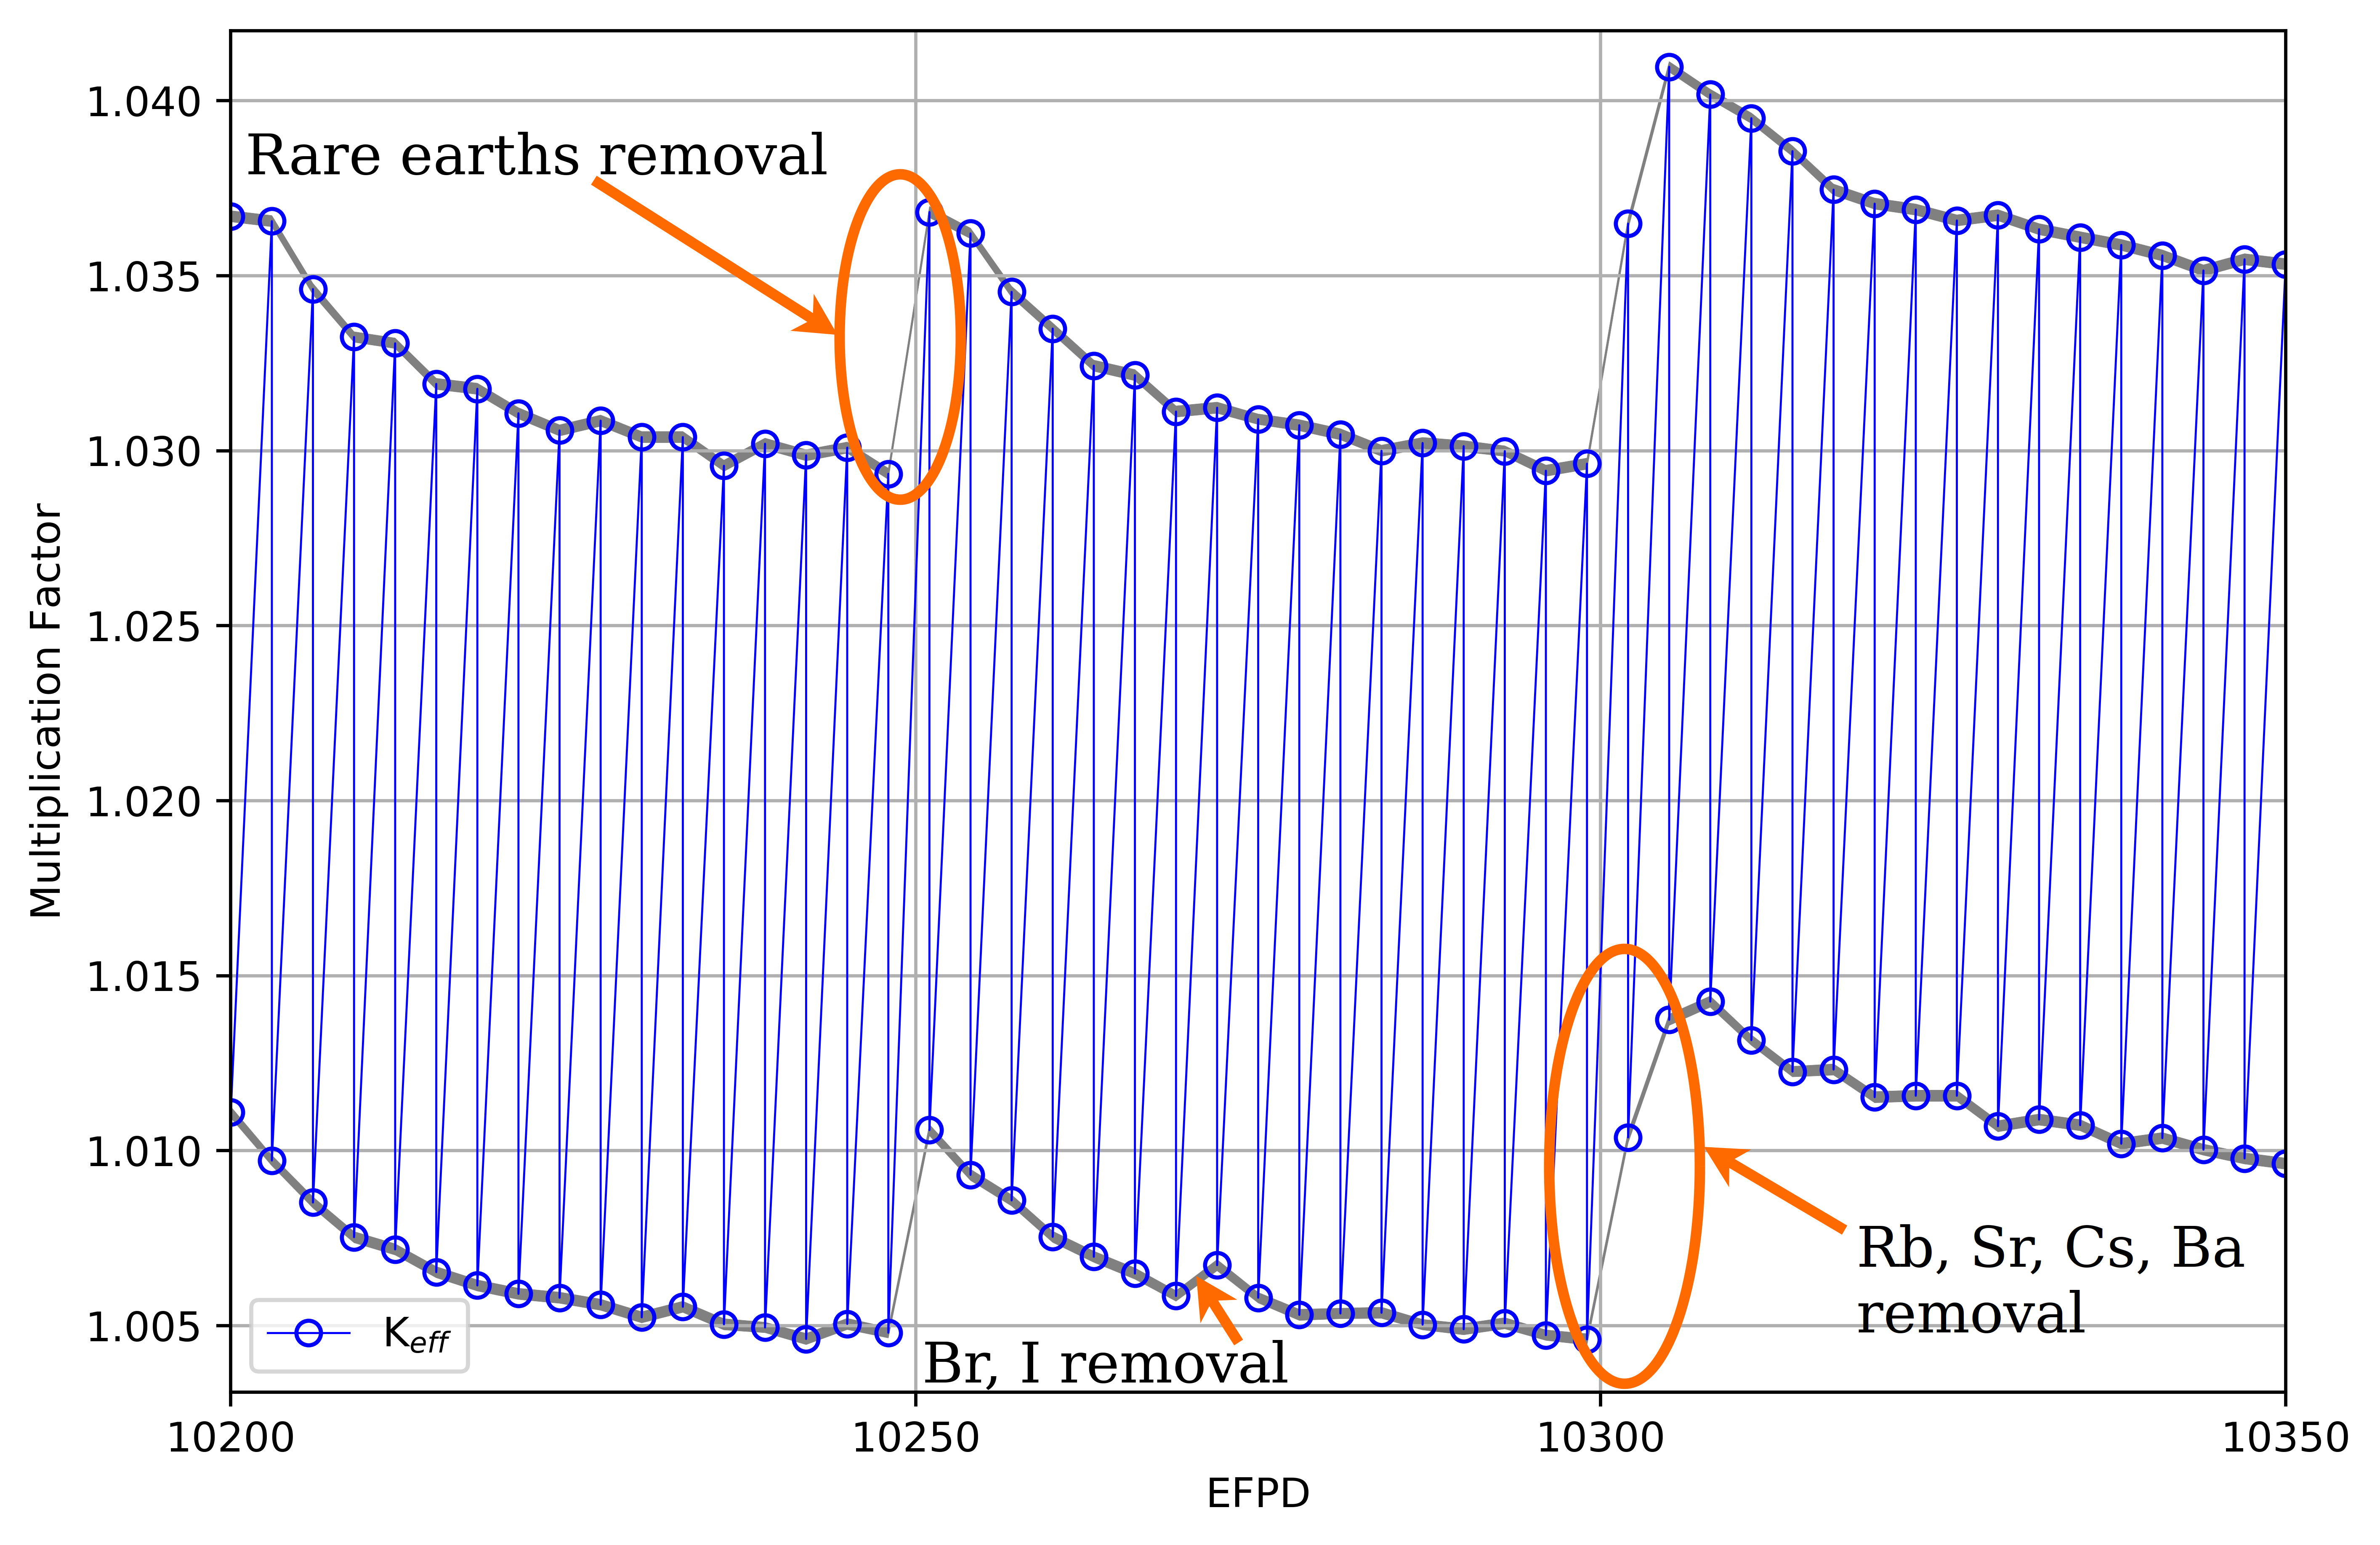
\includegraphics[width=\textwidth]{keff_zoomed.png}
  \caption{Zoomed effective multiplication factor for 150-EFPD time interval.}
  \label{fig:keff_zoomed}
\end{figure}

\subsection{Fuel salt composition dynamics}
The analysis of the fuel salt composition evolution provides more comprehensive 
information about the equilibrium state. Figure~\ref{fig:adens_eq} shows the number 
densities of major nuclides which have a strong influence on the reactor core 
physics. The concentration of $^{233}$U, $^{232}$Th, $^{233}$Pa, and $^{232}$Pa in 
the fuel salt change insignificantly after approximately 2500 days of operation. 
In particular, the $^{233}$U number density fluctuates by less than 0.8\% between
 16 and 20 years of operation. Hence, a quasi-equilibrium state was 
achieved after 16 years of reactor operation.
\begin{figure}[ht!] % replace 't' with 'b' to 
  \centering
  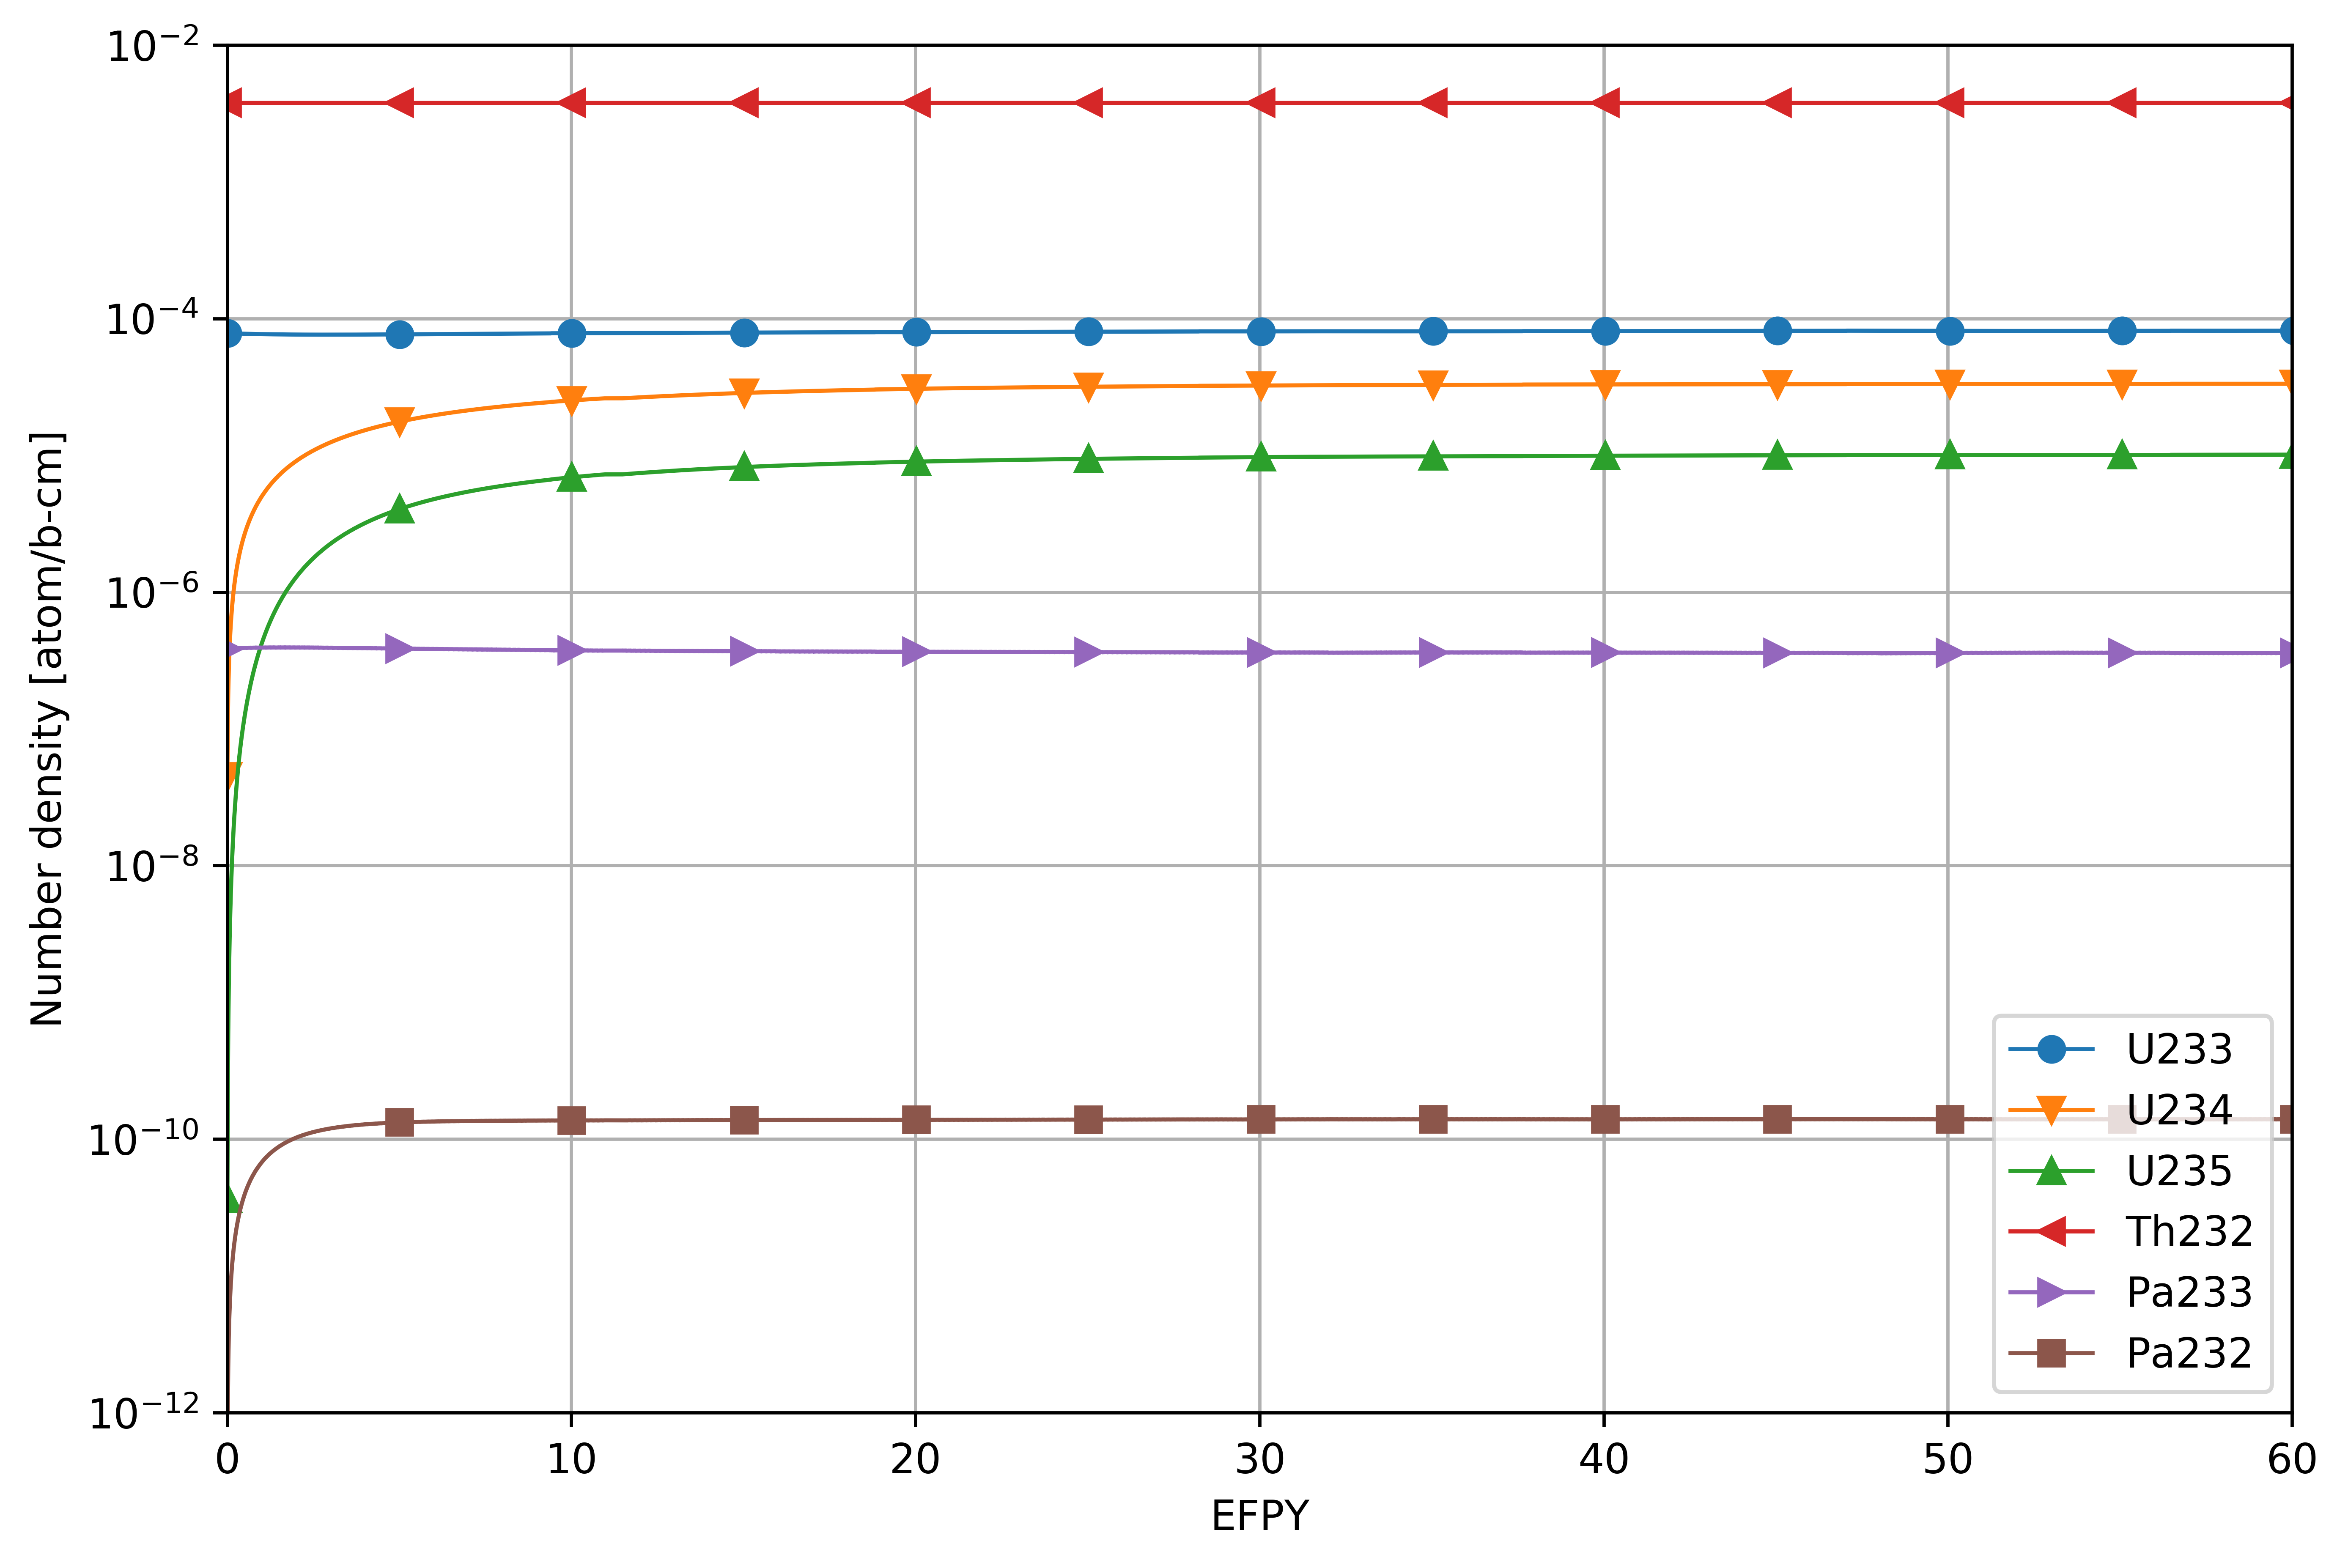
\includegraphics[width=\textwidth]{major_isotopes_adens.png}
  \caption{Number density of major nuclides during 60 years of reactor 
  operation.}
  \label{fig:adens_eq}
\end{figure}

\subsection{Neutron spectrum}
Figure~\ref{fig:spectrum} shows the normalized neutron flux spectrum for the 
full-core \gls{MSBR} model in the energy range from $10^{-8}$ to $10$ MeV. The 
neutron energy spectrum at equilibrium is harder than at startup due to 
plutonium and other strong absorbers accumulating in the core during reactor 
operation.  
\begin{figure}[ht!] % replace 't' with 'b'         to force it to 
  \centering
  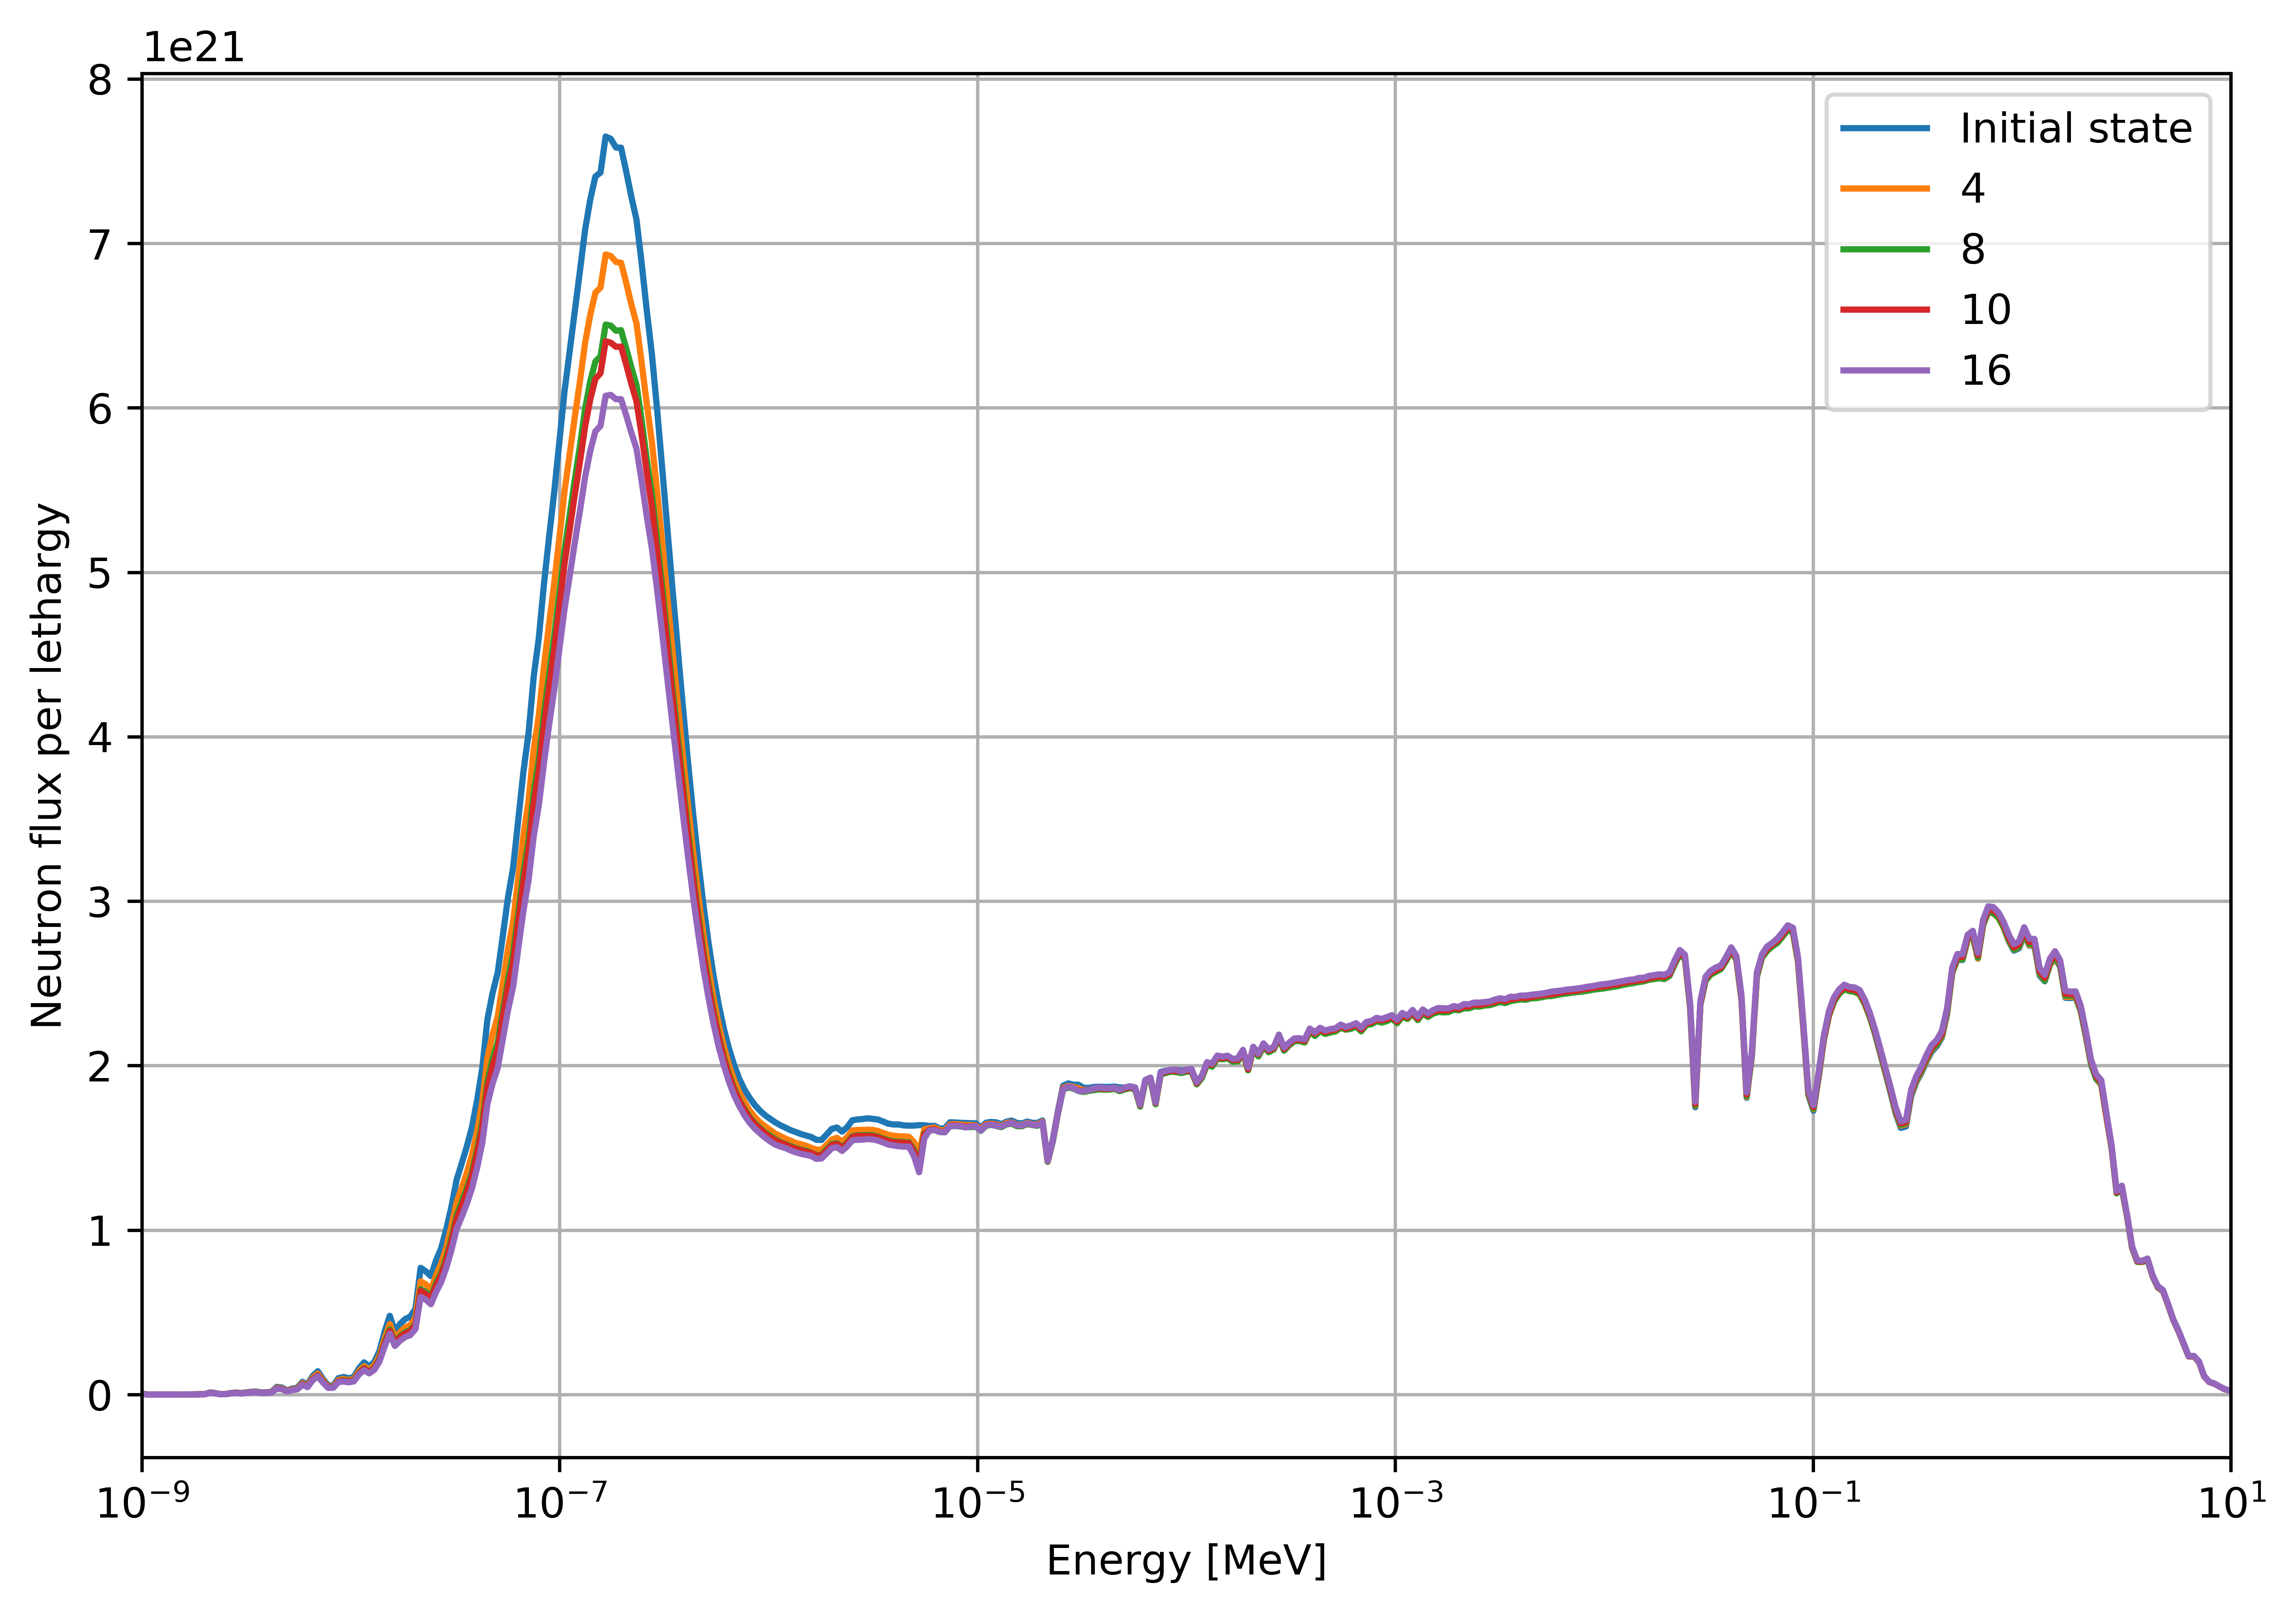
\includegraphics[width=\textwidth]{spectrum.png} \caption{The neutron flux energy 
  spectrum is normalized by unit lethargy and the area under the curve is normalized to 1 for initial and equilibrium fuel salt 
  composition.}
  \label{fig:spectrum}
\end{figure}

\begin{figure}[ht!] % replace 't' with 'b' to force it to 
  \centering
  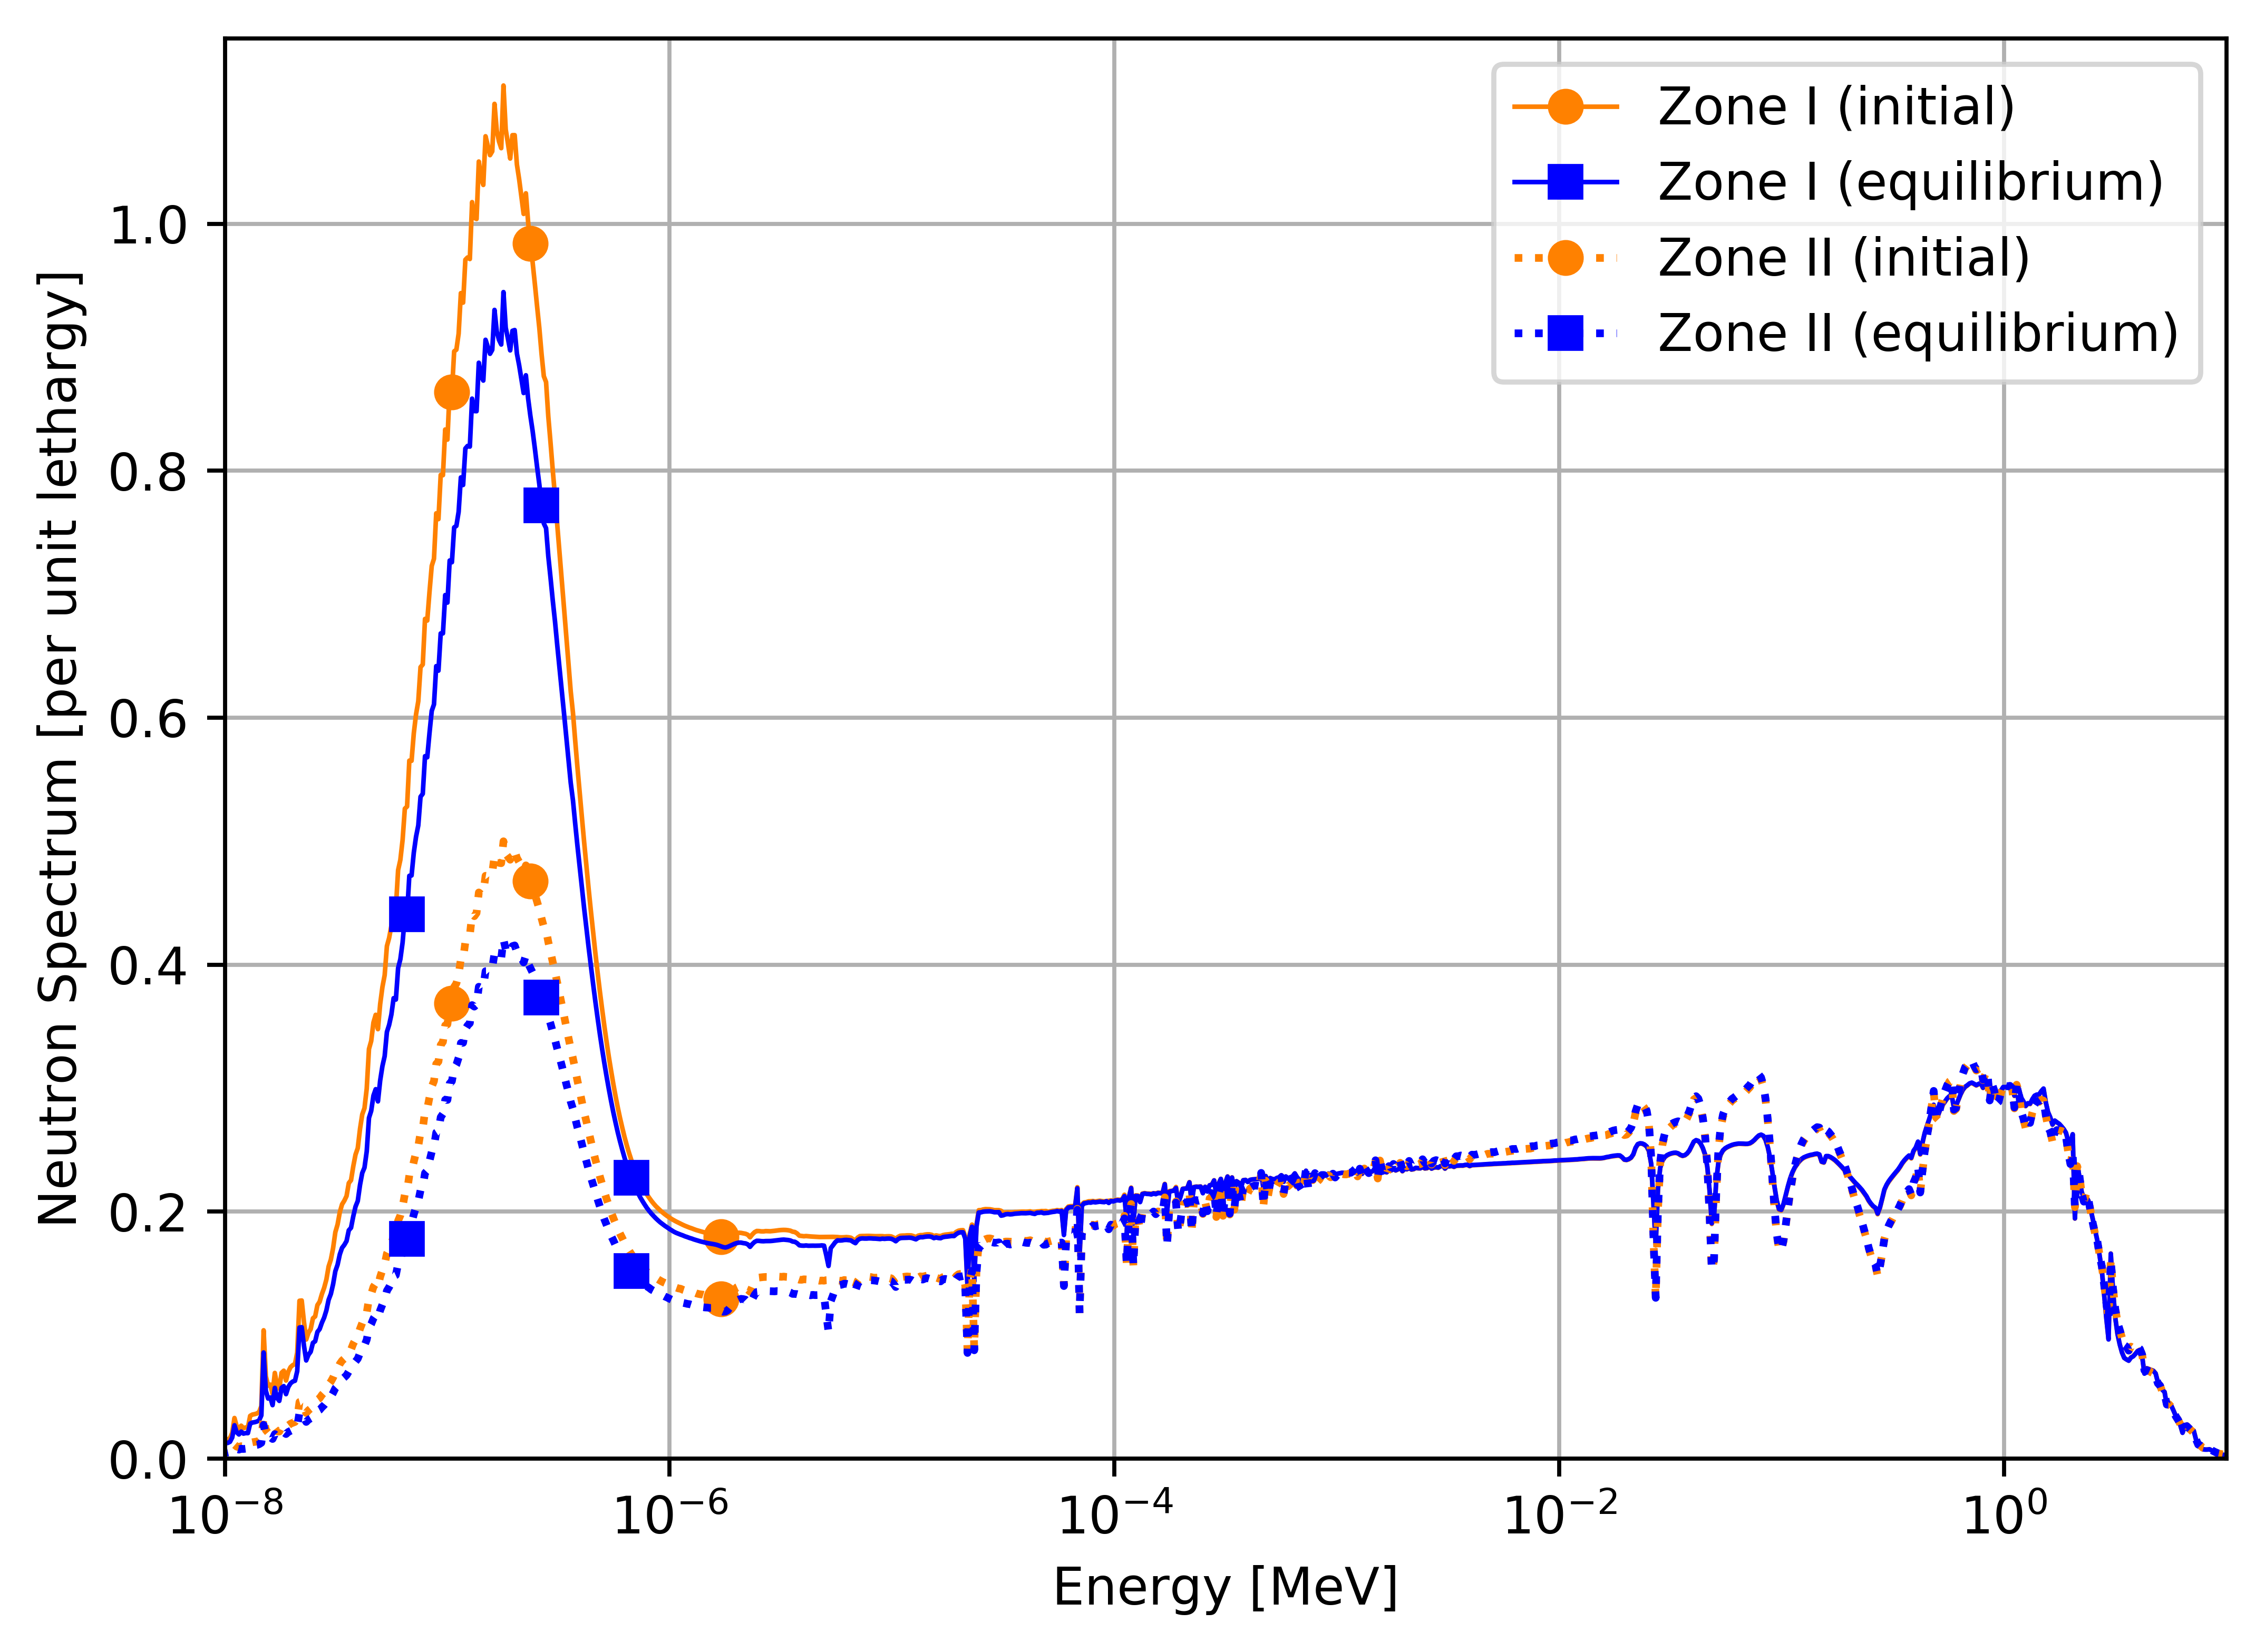
\includegraphics[width=\textwidth]{spectrum_zones.png} 
  \caption{The neutron flux energy spectrum in different core regions is normalized by 
unit lethargy and the area under the curve is normalized to 1 for the initial and equilibrium fuel salt composition.}
  \label{fig:spectrum_zones}
\end{figure}

\subsection{Neutron flux}
Figure~\ref{fig:radial_flux} shows the radial distribution of fast and thermal 
neutron flux for the both initial and equilibrium composition. 
\begin{figure}[ht!] % replace 't' with 'b' to force it to \centering
  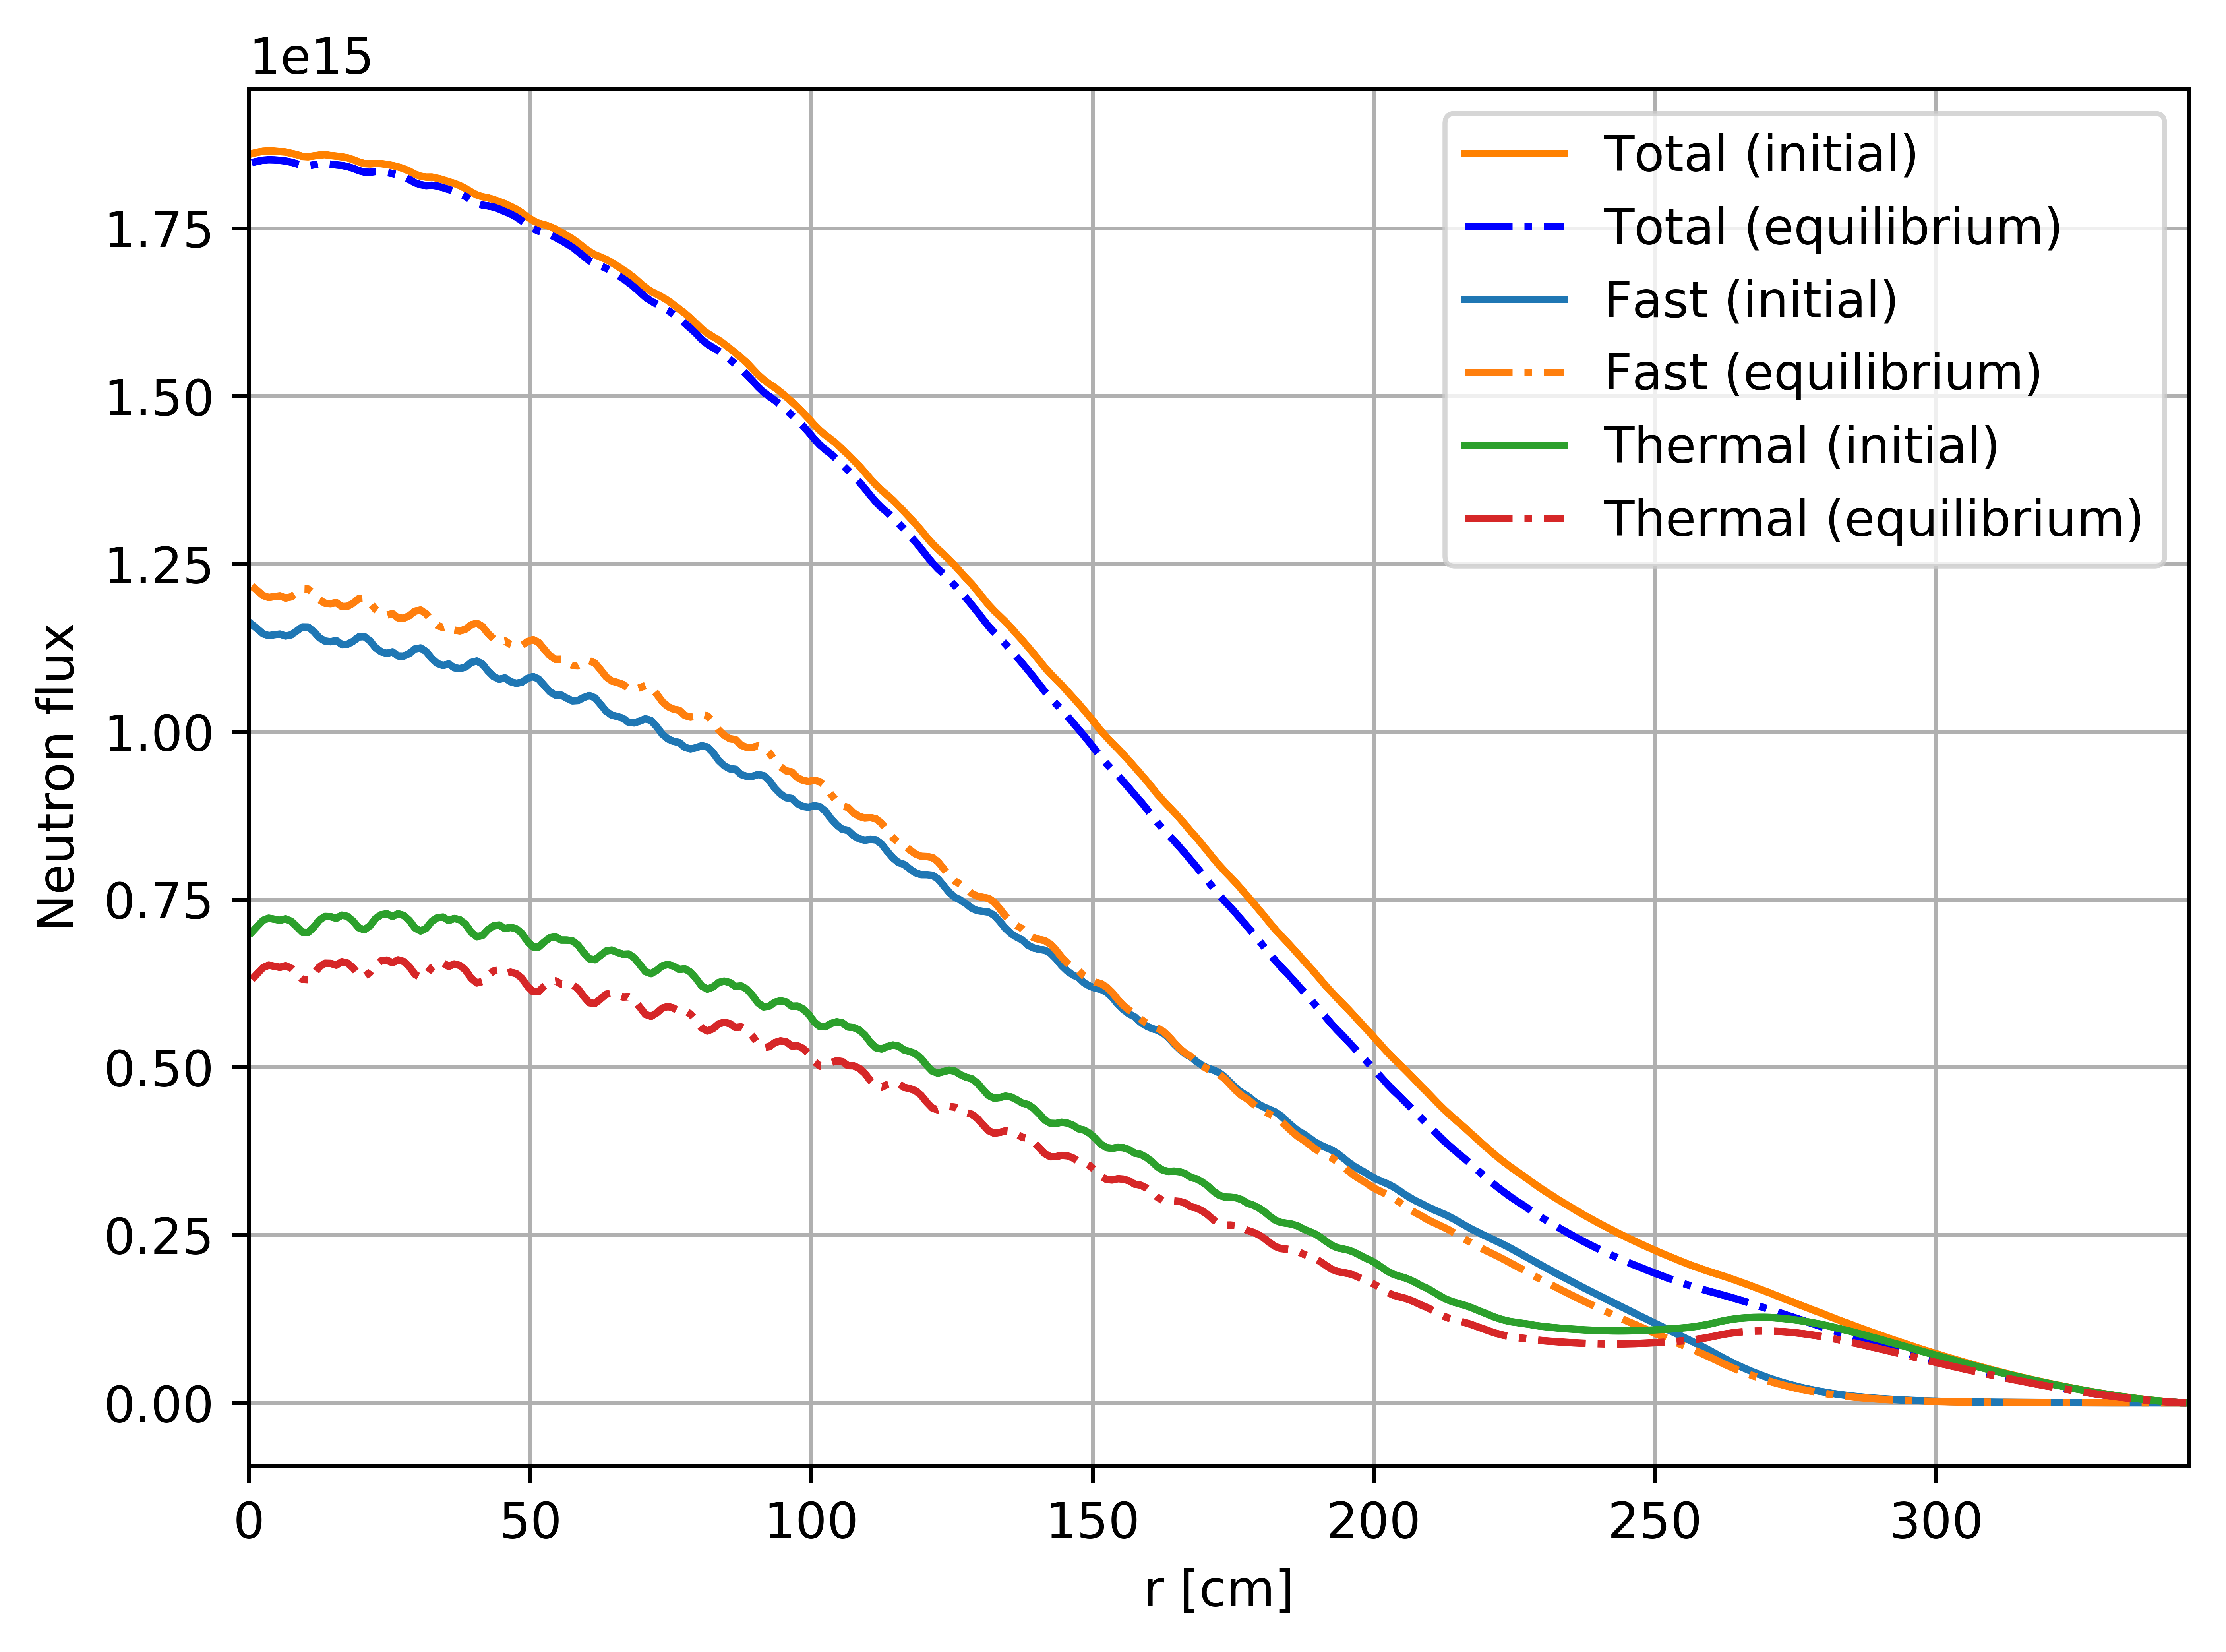
\includegraphics[width=\textwidth]{radial_flux.png} \caption{Radial neutron 
  flux distribution for initial and equilibrium fuel salt composition.}
  \label{fig:radial_flux}
\end{figure}

\subsection{Power and breeding distribution}
Table~\ref{tab:powgen_fraction} shows the power fraction in each zone for 
initial and equilibrium fuel compositions. Figure~\ref{fig:pow_den} reflects the 
normalized power distribution of the \gls{MSBR} quarter core for equilibrium fuel
 salt composition. For both the initial and equilibrium compositions, fission 
primarily occurs in the center of the core, namely zone I. The spectral shift 
during reactor operation results in slightly different power fractions at startup and 
equilibrium, but most of the power is still generated in zone I at equilibrium 
(table~\ref{tab:powgen_fraction}). 
%%%%%%%%%%%%%%%%%%%%%%%%%%%%%%%%%%%%%%%%
\begin{table}[ht!]
  \caption{Power generation fraction in each zone for initial and equilibrium 
  state.}
\begin{tabularx}{\textwidth}{ m | s | s } \hline
Core region      & Initial      & Equilibrium   \\   \hline
Zone I           & 97.91\%      & 98.12\%   \\
Zone II          & 2.09\%       & 1.88\%   \\ \hline
\end{tabularx}
  \label{tab:powgen_fraction}
\end{table}
%%%%%%%%%%%%%%%%%%%%%%%%%%%%%%%%%%%%%%%%%%%%%%%%%%%%%%%%%%%%%%%%%%%%%%%%%%%%%%%%
Figure~\ref{fig:breeding_den} shows the neutron capture reaction rate 
\begin{figure}[ht!] % replace 't' with 'b' to force it to \centering
  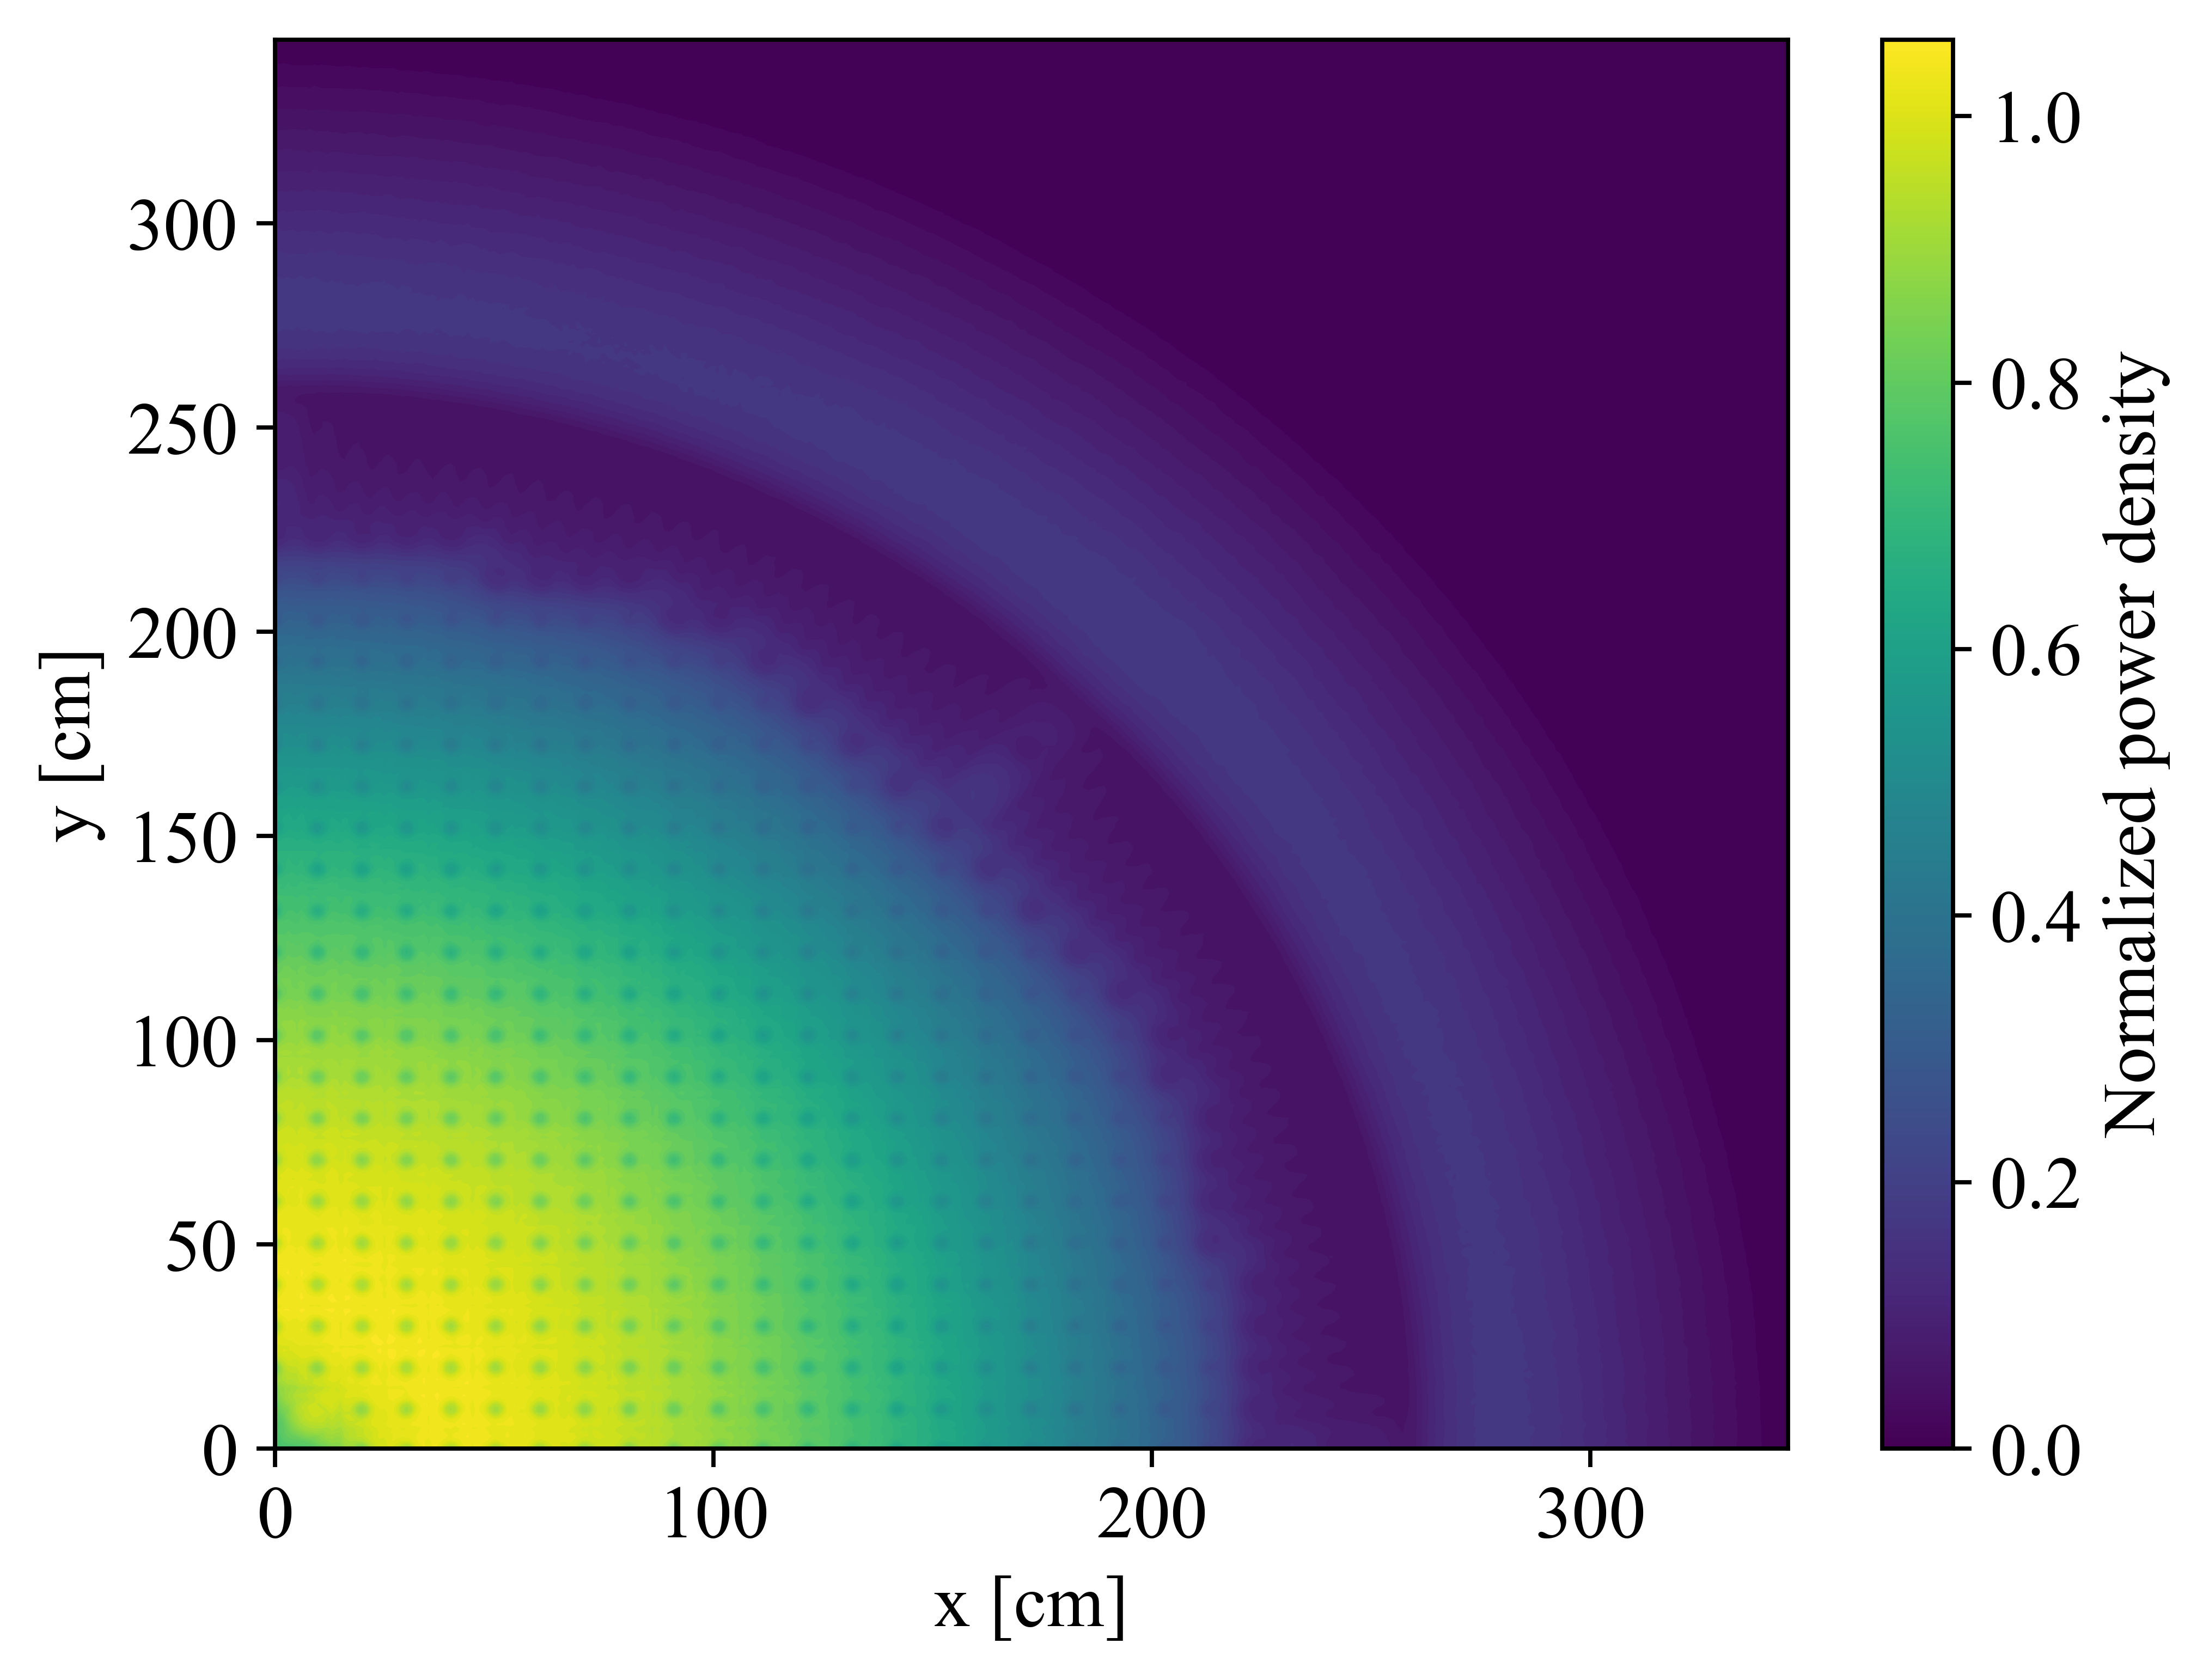
\includegraphics[width=\textwidth]{power_distribution_eq.png} 
  \caption{Normalized power density for equilibrium fuel salt 
  composition.}
  \label{fig:pow_den}
\end{figure}
\begin{figure}[ht!] % replace 't' with 'b' to force it to \centering
  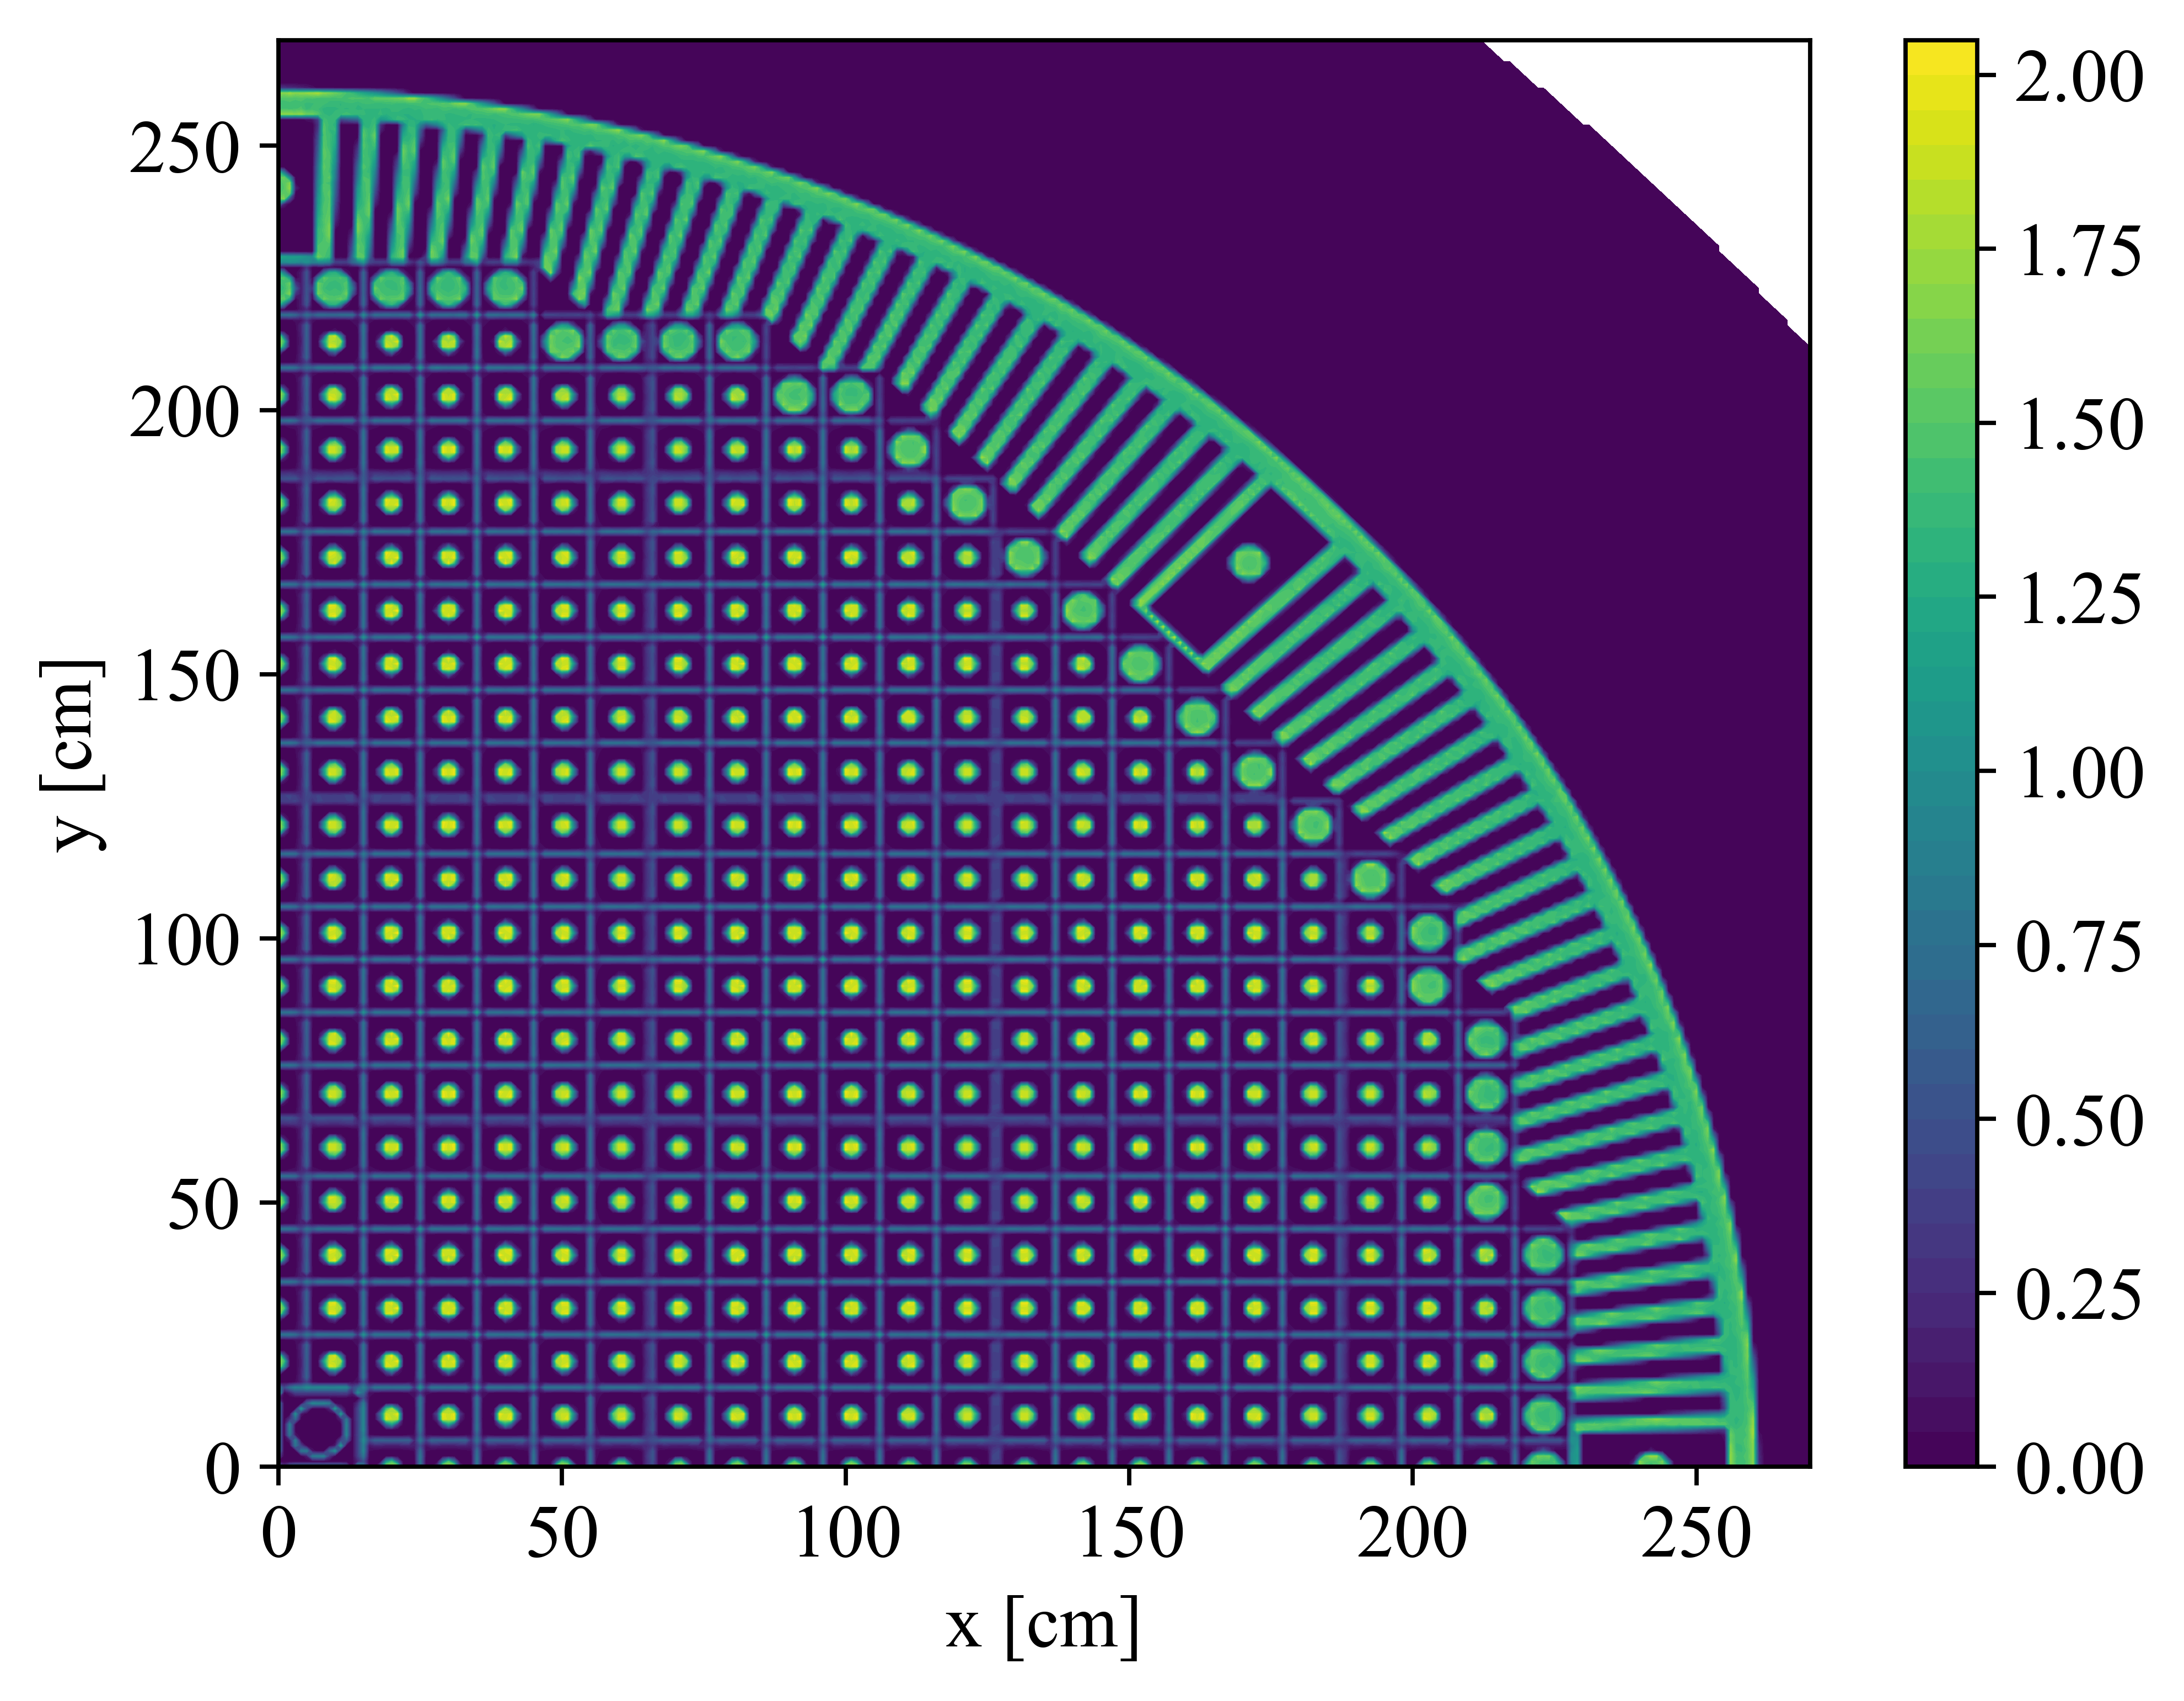
\includegraphics[width=\textwidth]{breeding_distribution_eq.png} 
  \caption{$^{232}$Th neutron capture reaction rate normalized by total flux 
  for equilibrium fuel salt composition.}
  \label{fig:breeding_den}
\end{figure}
\subsection{Temperature coefficient of reactivity}
Table~\ref{tab:tcoef} summarizes temperature effects on reactivity calculated 
in this work for both initial and equilibrium fuel compositions, compared 
with the original \gls{ORNL} report data \cite{robertson_conceptual_1971}. 
By propagating the $k_{eff}$  statistical error provided by SERPENT2, 
uncertainty for each temperature coefficient was obtained and appears in 
Table~\ref{tab:tcoef}. Other sources of uncertainty are neglected, such as cross section 
measurement error and approximations inherent in the equations of state 
providing both the salt and graphite density dependence on temperature.
 The main physical principle underlying the reactor 
temperature feedback is an expansion of heated material. When the fuel 
salt temperature increases, the density of the salt decreases, but at the same 
time, the total volume of fuel salt in the core remains constant because it is 
bounded by the graphite. When the graphite temperature increases, the density 
of graphite decreases, creating additional space for fuel salt. To determine 
the temperature coefficients, the cross section temperatures for the fuel and 
moderator were changed from 900K to 1000K. Three different cases were considered:
\begin{enumerate}
  \item Temperature of fuel salt rising from 900K to 1000K.
  \item Temperature of graphite rising from 900K to 1000K.
  \item Whole reactor temperature rising from 900K to 1000K.
\end{enumerate}
%%%%%%%%%%%%%%%%%%%%%%%%%%%%%%%%%%%%%%%%
\begin{table}[ht!]
  \caption{Temperature coefficients of reactivity for initial and equilibrium 
  state.}
\begin{tabularx}{\textwidth}{ X | r | r | r } \hline
Reactivity coefficient               & Initial         & Equilibrium     & Reference                                 \\ 
                                        & [pcm/k]         &  [pcm/k]        & (initial/equilibrium)\cite{li_optimization_2018} \tabularnewline  \hline
Doppler in fuel salt                    & $-4.70\pm0.159$ & $-5.30\pm0.186$ & 
\tabularnewline
Fuel salt density                       & $+1.19\pm0.155$ & $+2.93\pm0.186$ & 
\tabularnewline
Total fuel salt                         & $-3.67\pm0.157$ & $-2.62\pm0.189$ & 
\tabularnewline \hline
Doppler in graphite                     & $+2.00\pm0.158$ & $+0.85\pm0.188$ &          \tabularnewline
Total moderator (graphite)              & $+2.00\pm0.158$ & $+0.85\pm0.188$ & 
\tabularnewline \hline
Total core                              & $-1.45\pm0.159$ & $-2.04\pm0.186$ & $-2.0/-1.8$  \tabularnewline \hline
\end{tabularx}
  \label{tab:tcoef}
\end{table}
%%%%%%%%%%%%%%%%%%%%%%%%%%%%%%%%%%%%%%%%%%%%%%%%%%%%%%%%%%%%%%%%%%%%%%%%%%%%%%%%
In the first case, changes in the fuel temperature only impact fuel density. In 
this case, the geometry is unchanged because the fuel is a liquid. However, 
when the moderator heats up, both the density and the geometry change due to 
thermal expansion of the solid graphite blocks and reflector. Accordingly, the 
new graphite density was calculated using a linear temperature expansion 
coefficient of 1.3$\times10^{-6}$K$^{-1}$ \cite{robertson_conceptual_1971}. A new 
geometry input for SERPENT2, which takes into account displacement of graphite 
surfaces, was created based on this information. For calculation of 
displacement, it was assumed that the interface between the graphite reflector and vessel did not move,
 and that the vessel temperature did not change. This is the most reasonable assumption for
 the short-term reactivity effects because inlet salt is cooling graphite reflector and 
inner surface of the vessel.

The fuel temperature coefficient (FTC) is negative for both initial and 
equilibrium fuel compositions due to thermal Doppler broadening of the resonance 
capture cross sections in the thorium. A small positive effect of fuel density on 
reactivity increases from $+1.21$ pcm/K at reactor startup to $+1.66$ pcm/K for 
equilibrium fuel composition which has a negative effect on FTC magnitude during the 
reactor operation. This is in good agreement with earlier 
research \cite{robertson_conceptual_1971,park_whole_2015}. The moderator 
temperature coefficient (MTC) is positive for the startup composition and decreases 
during reactor operation because of spectrum hardening with fuel depletion. 
Finally, the total temperature coefficient of reactivity is negative for both 
cases, but decreases during reactor operation due to spectral shift. In 
summary, even after 20 years of operation the total temperature coefficient of 
reactivity is relatively large and negative during reactor operation (comparing 
with conventional PWR which has temperature coefficient about -1.71 pcm/$^\circ$F 
$\approx$ -3.08 pcm/K \cite{forget_integral_2018}), despite positive MTC, and 
affords excellent reactor stability and control.

\subsection{Six Factor Analysis}
The effective multiplication factor can be expressed using the following formula:
\begin{align*}
k_{eff} = k_{inf} P_f  P_t = \eta \epsilon p f P_f P_t
\end{align*}

Table~\ref{tab:six_factor} summarizes the six factors for both initial and 
equilibrium fuel salt composition. Using SERPENT2 and SaltProc, these factors and their statistical uncertainties
 have been calculated for both initial and equilibrium fuel salt composition (see 
Table~\ref{tab:msbr_tab}). The fast and thermal non-leakage probabilities 
remain constant despite the evolving neutron spectrum during operation. In 
contrast, the neutron reproduction factor ($\eta$), resonance escape 
probability ($p$), and fast fission factor ($\epsilon$) are considerably different between startup and 
equilibrium. As indicated in Figure~\ref{fig:spectrum}, the neutron spectrum is 
softer at the beginning of reactor life. Neutron spectrum hardening causes the fast 
fission factor to increase through the core lifetime. The opposite is true for the 
resonance escape probability. Finally, the neutron reproduction factor 
decreases during reactor operation due to accumulation of fissile plutonium 
isotopes.
%%%%%%%%%%%%%%%%%%%%%%%%%%%%%%%%%%%%%%%%
\begin{table}[hb!]
  \caption{Six factors for the full-core \gls{MSBR} model for initial and 
  equilibrium fuel composition.}
\begin{tabularx}{\textwidth}{ b | s | s } \hline
Factor  & Initial      & Equilibrium   \\ \hline
Neutron reproduction factor ($\eta$)     & $1.3960\pm.000052$     & 
        $1.3778\pm.00005$ \\ Thermal utilization factor (f)           & 
        $0.9670\pm.000011$     & $0.9706\pm.00001$ \\
Resonance escape probability (p)         & $0.6044\pm.000039$     & 
        $0.5761\pm.00004$ \\
Fast fission factor ($\epsilon$)         & $1.3421\pm.000040$     & 
        $1.3609\pm.00004$ \\
Fast non-leakage probability (P$_f$)     & $0.9999\pm.000004$     & 
        $0.9999\pm.000004$ \\
Thermal non-leakage probability (P$_t$)  & $0.9894\pm.000005$     & 
        $0.9912\pm.00005$ \\ \hline
\end{tabularx}
  \label{tab:six_factor}
\end{table}
%%%%%%%%%%%%%%%%%%%%%%%%%%%%%%%%%%%%%%%%%%%%%%%%%%%%%%%%%%%%%%%%%%%%%%%%%%%%%%%%
\subsection{Thorium refill rate and U233 production}
